\documentclass[12pt,a4paper]{scrartcl}
    \usepackage[utf8]{inputenc}
    \usepackage{amsmath}
    \usepackage{amsfonts}
    \usepackage{amssymb}
    \usepackage{graphicx}

    \usepackage[bottom = 1in, left = 0.5in, right = 0.5in, top = 1in]{geometry}

    \usepackage[english]{babel}
    \usepackage[autostyle]{csquotes}
    \usepackage{mathptmx}

    \usepackage[labelfont=bf]{caption}

    \usepackage[default, scale=0.95]{opensans}

    \usepackage[T1]{fontenc}

    \usepackage{fixltx2e}

    % \addto\captionsenglish{\renewcommand{\figurename}{Supplementary Fig.}}
    % \addto\captionsenglish{\renewcommand{\tablename}{Supplementary Table}}

    \title{Figures}
    \date{}

\begin{document}
\maketitle

\begin{figure}[h]
	\centering
	\includegraphics[scale = 1]{../../../graphs/fig1.pdf}
	\caption{Density plots showing the distribution of transmittance values measured by the ROV and the SUIT devices. Numbers on top of the gray boxes identify the stations. Dashed lines represent the 10\% transmittance threshold.}
\end{figure}

\clearpage
\newpage

\begin{figure}[h]
	\centering
	\includegraphics[scale = 1]{../../../graphs/fig2.pdf}
	\caption{Violin plots of primary production calculated from ROV and SUIT transmittance data. For SUIT data, mixing models were calculated using only transmittance~$\le$~10\% (see Fig. 1) whereas the under ice models were calculated using all transmittance data.}
\end{figure}

\clearpage
\newpage

\begin{figure}[h]
	\centering
	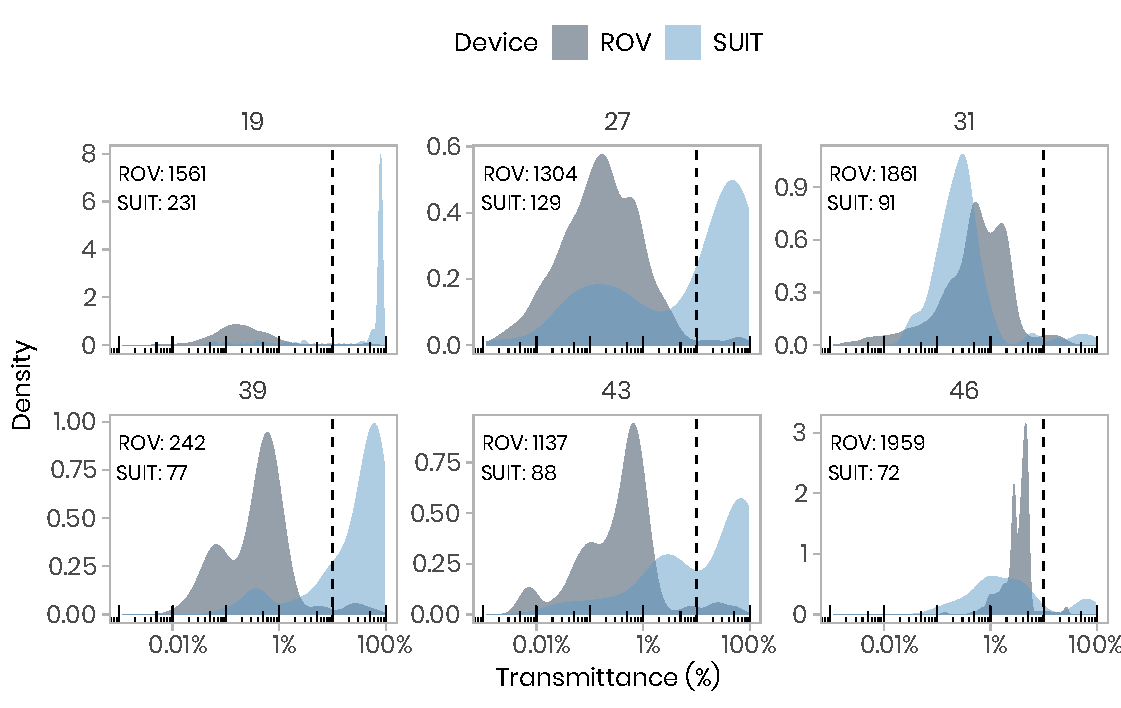
\includegraphics[scale = 1]{../../../graphs/fig3.pdf}
	\caption{Averaged vertical profiles of daily primary production. For SUIT data, mixing models were calculated using only transmittance $\le$ 0.1 whereas the under ice models were calculated using all transmittance data. Note the varying scales among stations.}
\end{figure}

\clearpage
\newpage

\begin{figure}[h]
	\centering
	\includegraphics[scale = 1]{../../../graphs/fig4.pdf}
	\caption{xxx}
\end{figure}

\end{document}
